\section{Theory}

\subsection{Molecular Dynamics Simulation}

Molecular Dynamics (MD) is a computational method used for molecular modeling and simulation in which the interactions between atoms and molecules are iteratively calculated to predict the behavior of a system over time. In order to calculate the forces acting on each atom, a potential energy function \(V\) is used, which describes the interactions between atoms. Besides classical force-fields, which are based on empirical formulas, machine learning interatomic potentials (MLIPs) have emerged as a powerful alternative, providing a more accurate representation of the potential energy surface (PES) by learning from quantum mechanical calculations.
Commonly a equation of motion has to be solved, which uses Newton's second law of motion:
\begin{equation}
    m \frac{d^2 \textbf{r}}{dt^2} = -\nabla V(\textbf{r})
\end{equation}
where \(m\) is the mass of the atom, \(\textbf{r}\) is the position vector of the atom, and \(\nabla V\) is the gradient of the potential energy function with respect to the position. With a suitable numerical integration method, such as the Verlet algorithm, the positions and velocities of the atoms can be updated iteratively to simulate the dynamics of the system over time.
After a simulation step, the forces acting on each atom are recalculated based on the updated positions, and the process is repeated until the desired simulation time is reached.
The simulation typically runs in with the constrains of a specific ensemble, such as the microcanonical (NVE), canonical (NVT) or isothermal-isobaric (NPT) ensemble, which defines the thermodynamic conditions of the system.
The ensemble used in the project is a NVT ensemble, where the number of particles \(N\), the volume \(V\) and the temperature \(T\) are kept constant. This is achieved by using a thermostat, such as the Langevin thermostat, which adds a stochastic term to the equations of motion to control the temperature of the system. Other common thermostats include the Nosé-Hoover thermostat and the Berendsen thermostat, each with its own advantages and disadvantages in terms of accuracy and computational efficiency.
The Langevin thermostat, combines deterministic and stochastic forces to maintain the desired temperature. This has a downside of changing the dynamics of the system resulting in a non-newtonian trajectory. Therefore dynamic properties, such as diffusion coefficients, should not be calculated from a NVT simulation with a Langevin thermostat.
In order to evaluate thermodynamic properties, the ensemble average (average over all microstates of the system) is calculated. The output of a MD simulation is typically a long trajectory of microstates evolving over time.
The ergodic hypthesis connects the time average of a property to its ensemble average, allowing us to compute thermodynamic properties from a single trajectory, provided that the system is ergodic and the simulation time is sufficiently long.

\subsection{Quantum Mechanical Foundations}

A quantum mechanical system is generally described by a wavefunction \(\Psi\) and the time-dependent Schrödinger equation:
\begin{equation}
    i \hbar \frac{\partial \Psi}{\partial t} = \hat{H} \Psi
\end{equation}
where \(\hbar\) is the reduced Planck constant, and \(\hat{H}\) is the Hamiltonian operator, which represents the total energy of the system. For a single particle in a potential \(V(\textbf{r})\), the Hamiltonian can be expressed as:
\begin{equation}
    \hat{H} = -\frac{\hbar^2}{2m} \nabla^2 + V(\textbf{r})
\end{equation}
where \(m\) is the mass of the particle, and \(\nabla^2\) is the Laplacian operator, which accounts for the kinetic energy of the particle.
Because this is to complex to solve for many-body systems, the Born-Oppenheimer approximation is often used, which separates the electronic and nuclear degrees of freedom, based on the difference in their masses.
This reduces the problem to solving the electronic Schrödinger equation for fixed nuclear positions.
Another approximation is the linear combination of atomic orbitals (LCAO), which expresses the molecular orbitals as a linear combination of atomic orbitals. Combined with the Hartree-Fock method, which approximates the many-electron wavefunction as a single Slater determinant, this allows for the calculation of electronic structure and properties of molecules.

In order to simulate a quantum mechanical system, the Density Functional Theory (DFT) is often used, which is a computational quantum mechanical method that describes the electronic structure of many-body systems in terms of the electron density \(\rho(\textbf{r})\) rather than the wavefunction.
The Hohenberg-Kohn theorems state that the ground-state properties of a many-electron system are uniquely determined by the electron density, and that there exists a universal functional \(E[\rho]\) that can be used to calculate the total energy of the system.
The Kohn-Sham equations transform the many-electron problem into a set of single-particle equations in a self-consistent field (SCF) approach, where the electron density is iteratively updated until convergence is achieved.
The result is a single particle potential:
\begin{equation}
    V_{\text{s}} (\mathbf{r}) = V_{\text{ext}} (\textbf{r}) + V_H (\textbf{r}) + V_{\text{xc}} (\textbf{r})
\end{equation}
where \(V_{\text{ext}}\) is the external potential, \(V_H\) is the Hartree potential, and \(V_{\text{xc}}\) is the exchange-correlation potential, which accounts for the many-body effects of electron-electron interactions.
There are many different exchange-correlation functionals, such as the Local Density Approximation (LDA), the Generalized Gradient Approximation (GGA) and hybrid functionals, which combine DFT with Hartree-Fock exchange.

\subsection{Dispersion Correction}
Because DFT is a mean-field theory, it fails to capture long-range dispersion interactions, which are crucial for accurately describing the behavior of many systems. In order to account for these interactions, dispersion correction methods such as the Grimme-D3 methods can be applied after the DFT calculation. The D3 method adds an empirical dispersion energy term to the total energy calculated by DFT, which is based on a pairwise additive model of dispersion interactions between atoms.
The energy correction is calculated as:
\begin{equation}
    E_{\text{disp}} = -\sum_{i<j} \sum_{N} \left(\frac{C_6^{ij}}{R^6_{ij, L}}f_{d, 6}(R_{ij, L}) + \frac{C_8^{ij}}{R^8_{ij, L}}f_{d, 8}(R_{ij, L})\right)
\end{equation}
where \(C_6^{ij}\) and \(C_8^{ij}\) are the dispersion coefficients for the atom pair \(i,j\), \(R_{ij, L}\) is the distance between the atoms, and \(f_{d, n}(R)\) is a damping function that prevents the correction from diverging at short distances.
Dispersion corrections are independent of the underlying electron density.

\subsection{Neural Networks}
The modern Neural Networks (NNs) are based on a mathematical model of the neuron, a so-called artificial neuron or perceptron.
This neuron receives multiple inputs \(\textbf{x}\) and applies a learnable weight \(w_{i}\) to each input, sums them up and adds a bias \(b\) to produce an output \(y\).
This information is then passed through a non-linear activation function \(f\) to introduce non-linearity into the model, allowing it to learn complex patterns in the data.
\begin{equation}
    y = f\left( \sum_{i=1}^{n} w_{i} x_{i} + b \right) = f ( \textbf{x} \cdot \textbf{w} + b )
\end{equation}
A common activation function is the Rectified Linear Unit (ReLU), defined as \(f(x) = \max(0, x)\).
In order to advance in high-dimensional problems, multiple layers of neurons are stacked together to form a deep neural network.
The arangement of these layers, called architecture, can vary widely and changes the way the network learns and processes information.
Usual architectures include feedforward networks, convolutional neural networks (CNNs) and recurrent neural networks (RNNs).
\begin{figure}
    \centering
    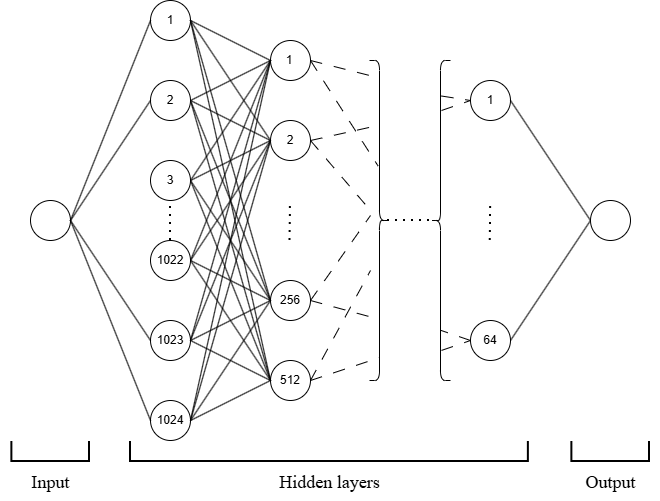
\includegraphics[width=0.8\textwidth]{images/NN.png}
    \caption{Schematic representation of a simple feedforward neural network with several hidden layers.}
\end{figure}

A better way to represent the architecture of a neural network is through matrix operations.
A hidden layer \(l\) with \(m\) neurons receives an input vector \(\textbf{a}^{(l-1)}\) of size \(n\) from the previous layer, applies a weight matrix \(\textbf{W}^{(l)}\) of size \(m \times n\) and a bias vector \(\textbf{b}^{(l)}\) of size \(m\), and produces an output vector \(\textbf{a}^{(l)}\) of size \(m\).
\begin{equation}
    \textbf{a}^{(l)} = f\left(\textbf{W}^{(l)} \cdot \textbf{a}^{(l-1)} + \textbf{b}^{(l)}\right)
\end{equation}

Stacking multiple layers allows the network to become a highly complex and non-linear function.
The combination of the non-linear activation functions and the learnable parameters (weights and biases) enables the network to approximate a wide variety of functions, making it a powerful tool for tasks such as classification, regression, and generative modeling.

\subsection{Training a Neural Network}
In order to improve the performance of a NN, it needs to be trained on a dataset. This process is realized by determining the optimal network parameters (weights \(\textbf{W}\) and biases \(\textbf{b}\)) that minimize a loss function \(\mathcal{L}\), which quantifies the difference between the predicted output and the true output.
A simple example of a loss function is the mean squared error (MSE) for regression tasks:
\begin{equation}
    \mathcal{L}_{MSE}(\hat{y}, y) = \frac{1}{N} \sum_{i=1}^{N} (\hat{y}_{i} - y_{i})^2
\end{equation}
where \(\hat{y}\) is the predicted output, \(y\) is the true output, and \(N\) is the number of samples in the dataset.

\begin{figure}
    \centering
    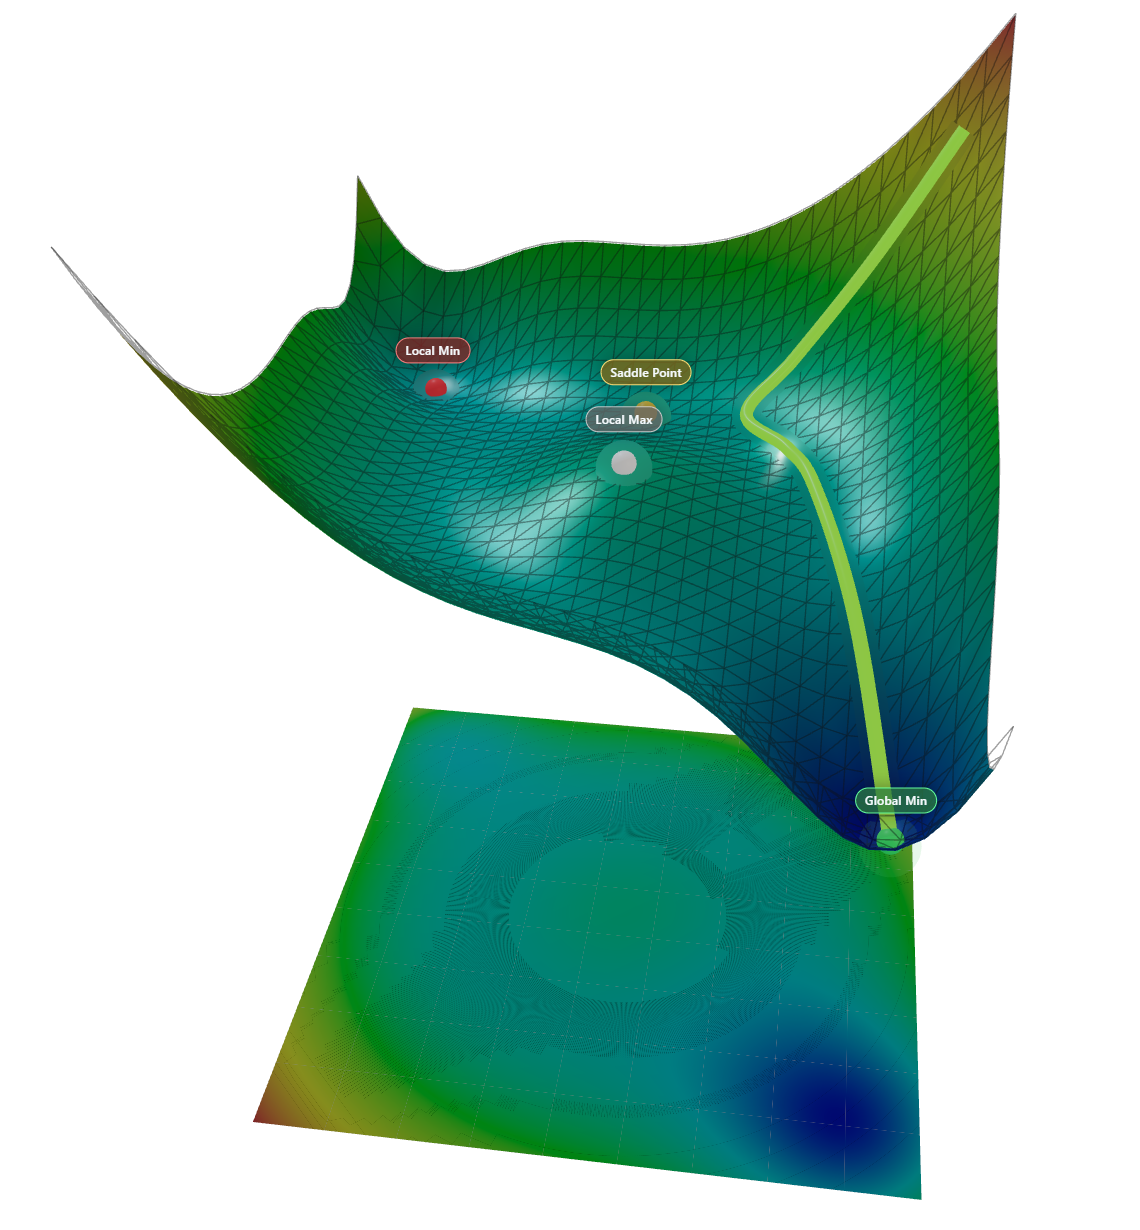
\includegraphics[width=0.8\textwidth]{images/PES.png}
    \caption{Schematic representation of the training process of a neural network, where the loss function is minimized by adjusting the weights and biases.}
\end{figure}

\subsection{Descriptors}
In order to reduce the complexity of the input data and ensure a consistent input vector size, descriptors are used to represent the atomic environment in a fixed-size vector.
A descriptor transforms the atomic environment into a numerical representation that captures the relevant information for the task at hand, such as the local geometry and chemical composition.
The Gaussian Moment Neural Network Input  descriptor (short:GMNN-descriptor, used in this project) ensures that the input vector remains invariant under:
\begin{itemize}
    \item Translation: The descriptor does not change if the entire system is shifted in space.
    \item Rotation: The descriptor remains unchanged if the system is rotated in space.
    \item Permutation: The descriptor is invariant to the permutation of identical atoms.
\end{itemize}
This also allows the network to learn the underlying physics of the system, rather than just memorizing specific configurations, which improves the generalization of the model to unseen data.


\subsection{Local Atomic Energy Partitioning}
A essential of an MLIP is that the energies are calculated on a local atomic level, the total energy of the system is a derived quantity. Behler and Parinello intriduced the concept of local atomic energy partitioning, stating that the total energy of a system can be decomposed into contributions from individual atoms, which depend on their local environment.
\begin{equation}
    E_{\text{total}} = \sum_{i=1}^{N} E_{i}
\end{equation}
where \(E_{\text{total}}\) is the total energy of the system, \(N\) is the number of atoms, and \(E_{i}\) is the local atomic energy contribution from atom \(i\).
One of the property-heads of the NN in this project predicts these local atomic energy contributions, which can then summed up to obtain the total energy of the system.

\subsection{The \textit{apax} Model Architecture}
The \textit{apax} model architecture allows a single network to predict not only different properties, but also allows the prediction of different atomic species. The information about the atomic species is encoded in the learnable parameters.

The forces needed for the MD simulation are calculated via Automatic Differentiation (AD), which allows the forces to be obtained from the energy predictions without the need for a separate force head in the network. The forces are therefore calculated analytically ensuring that they are consistent with the energy predictions, which is crucial for the stability and energy conservation of the MD simulation.

In order to improve the performance of the model, a loss function has to be defined, which quantifies the difference between the predicted properties and the true properties. A common choice for the loss function is the mean squared error (MSE):
\begin{equation}
    \mathcal{L} = \frac{1}{N} \sum_{i=1}^{N} \left( w_E (E_i - \hat{E}_i)^2 + w_F \sum_{j=1}^{3N} \|F_{ij} - \hat{F}_{ij}\|^2 \right)
\end{equation}
where \(N\) is the number of configurations, \(E\) and \(F\) are the predicted and true energies and forces, and \(w_E\), \(w_F\) are the weights for the energy and forces to the loss function, respectively.

\subsection{Uncertainty Quantification}

In order to assess the uncertainty of the model at a current simulation step, a shallow ensemble can be used to quantify the uncertainty of the predictions. With a shared backbone in the model but randomly initialized last layers, the ensemble can provide a measure of the uncertainty by evaluating the variance of the predictions across the ensemble members. The uncertainty \(sigma_x\) for a property \(x\) can be calculated as:
\begin{equation}
    \sigma_x = \sqrt{\frac{1}{M-1} \sum_{m=1}^{M} (x_m - \bar{x})^2}
\end{equation}
where \(M\) is the number of ensemble members, \(x_m\) is the prediction from the \(m\)-th ensemble member, and \(\bar{x}\) is the mean prediction across the ensemble.
This uncertainty can be used to identify configurations where the model is less confident, which can be useful for active learning strategies, where new data points can be added to the training set to improve the model's performance in those regions of the configuration space.

\section{Measurements}

\subsection{Diffusion Coefficient}

A quantitative measure of the diffusion of particles in a system is the diffusion coefficient \(D\). Fick's first law relates the flux of particles \(J\) to the concentration gradient \(\nabla C\) through the diffusion coefficient:
\begin{equation}
    J = -D \nabla C.
\end{equation}
The negative sign indicates that particles diffuse from regions of higher concentration to regions of lower concentration. The mean squared displacement (MSD) is defined as an ensemble-averaged squared distance that a particle travels over time \(t\). The Einstein relation connects the diffusion coefficient to the MSD:
\begin{equation}
    \lim_{t\to\infty} \text{MSD}(t) = 2nDt
\end{equation}
where \(n\) is the dimensionality of the system (e.g., \(n=3\) for three-dimensional space).
In practice we calculate the MSD by finding the slope \(m\) of the mean squared displacement as a function of time and then using the relation:
\begin{equation}
    D = \frac{m}{2n}
\end{equation}
The velocity autocorrelation function (VACF) is another tool to analyze the dynamics of particles in a system.
\begin{equation}
    D = \frac{1}{3} \int_{0}^{\infty} \langle \mathbf{v}(0) \cdot \mathbf{v}(t) \rangle dt
\end{equation}
The diffusion coefficient can be calculated by using the Stokes-Einstein relation, which relates the diffusion coefficient to the temperature \(T\) and the viscosity \(\eta\) of the medium:
\begin{equation}
    D = \frac{k_B T}{6 \pi \eta r}
\end{equation}
where \(k_B\) is the Boltzmann constant, and \(r\) is the radius of the diffusing particle. This relation assumes that the particle is spherical and that the medium is a continuous fluid with a well-defined viscosity.

\subsection{Radial Distribution Function}

The Radial Distribution Function (RDF), can be used to analyze the structure of a system by providing information about the probability of finding a particle at a certain distance from a reference particle. The RDF \(g(r)\) is defined as:
\begin{equation}
    g(r) = \frac{\rho(r)}{\rho_0}
\end{equation}
where \(\rho(r)\) is the instantaneous density at a distance \(r\) from a reference particle, and \(\rho_0\) is the average density of the system.
A RDF value of \(g(r) = 1\) indicates that the density at distance \(r\) is equal to the average density, while values greater than 1 indicate a higher density (i.e., more particles are found at that distance), and values less than 1 indicate a lower density (i.e., fewer particles are found at that distance).
A correct RDF is crucial for accurately for assessing a system, if the RDF is not correct but other properties are, chances are that the correct properties are just a result of error cancellation and the model is not generalizing well to unseen data.